% Indicate the main file. Must go at the beginning of the file.
% !TEX root = ../main.tex

%----------------------------------------------------------------------------------------
% CHAPTER TEMPLATE
%----------------------------------------------------------------------------------------


\chapter{System Overview} % Main chapter title

\label{ChapterSystemOverView} % Change X to a consecutive number; for referencing this chapter elsewhere, use \ref{ChapterX}

%----------------------------------------------------------------------------------------
% SECTION 1
%----------------------------------------------------------------------------------------

\section{Overview of the System}

\begin{figure}[ht]
    \centering
    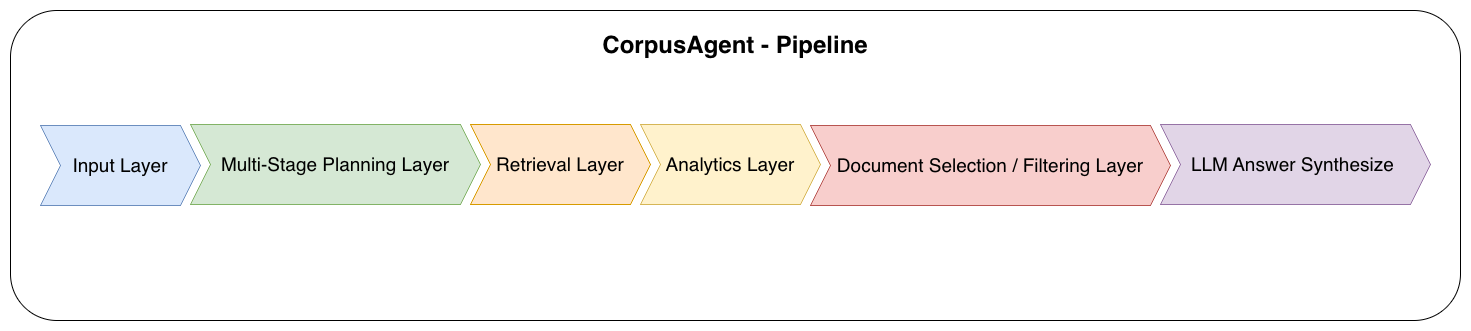
\includegraphics[width=1\textwidth]{Figures/Pipeline-Overview.png}
    \caption{Pipeline Overview}
    \label{fig:pipeline-overview}
\end{figure}

This thesis proposes a modular, multi-stage processing pipeline as illustrated in Figure \ref{fig:pipeline-overview}. The Pipeline of the CorpusAgent system is designed to answer complex, temporally-aware analytic questions over a large corpus of documents, specifically news articles. With such large datasets, it is infeasible to load all data into a large language model (LLM) prompt due to context length limitations. Therefore, the system breaks down the processing into several stages, each handled by specialized modules. Each of these layers is responsible for a specific transformation or decision step.

The core idea behind this architecture is to separate planning, retrieval, analysis, filtering and synthesis into independent stages. The separation of these stages allows for better scalability, maintainability, and the ability to swap out components as needed. Each layer incrementally refines the data, starting from a raw user query, progressing through structured retrieval and analytics processing and culminating in a final synthesized answer.

As this concept of ours is still experimental, we tried to structure the system as modularly as possible, so that individual components of the pipeline can be replaced or improved independently with different be it retrieval strategies, LLM models, or analytic techniques. The following section will describe each of these layers in detail, explaining their roles, inputs, outputs, and interactions with other components in the system.


%-----------------------------------
% Pipeline Layers
%-----------------------------------
\section{Pipeline Layers}

The CorpusAgent pipeline is composed of a sequence of logically separated layers, each responsible for a specific aspect of the overall processing workflow. The layers are executed in a predefined order, where the output of one layer serves as the input for the next. This layered design allows complex analytical tasks to be decomposed into smaller, more manageable steps, improving transparency and enabling targeted evaluation of individual components.

In the following subsections, each pipeline layer is described in detail. For each layer, its purpose, inputs, outputs, and interactions with other layers are explained.

%-----------------------------------
% Input Layer
%-----------------------------------
\subsection{Input Layer}

\begin{figure}[ht]
    \centering
    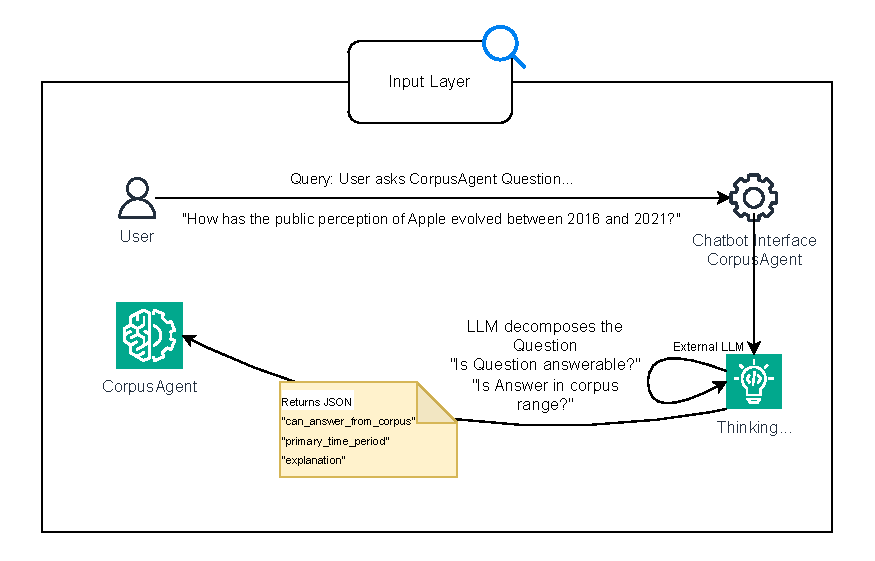
\includegraphics[width=1\textwidth]{Figures/input-layer.pdf}
    \caption{Input Layer}
    \label{fig:input-layer}
\end{figure}

The entry point of the CorpusAgent system is the Input Layer, as illustrated in Figure \ref{fig:input-layer}. It is responsible for receiving user queries, validating them, and performing any necessary preprocessing before passing them on to the subsequent layers.

The interaction begins when a user submits a natural language question through the chatbot interface of our CorpusAgent system. These questions are typically high-level analytical queries that may span over mutliple years and require aggregation or interpretation over a large corpus of documents. 

Upon receiving a query, the Input Layer forwards it to an either external or internal Large Language Model (LLM) for an initial reasoning step. At this stage, the LLM does not attempt to generate a final answer. Instead, it performs a lightweight decomposition and feasibility assessment of the query. Specifically, it evaluates whether the question falls within the temporal and thematic scope of the indexed data.

The motivation behind this design decision is to introduce an explicit reasoning and validation step at the very beginning of the pipeline. By performing an initial feasibility assessment, the system can identify questions that cannot be meaningfully answered using the available corpus, for example due to missing temporal coverage or insufficient data. This early filtering prevents unnecessary downstream processing and ensures that subsequent pipeline stages operate only on well-scoped and answerable queries.

The outcome of the assessment is a structured JSON format containing whether the question is answerable, the primary time period of interest and a short explanation justifying the decision. 



%-----------------------------------
% Multi-Stage Planning Layer
%-----------------------------------

\subsection{Multi-Stage Planning Layer}

\begin{figure}[ht]
    \centering
    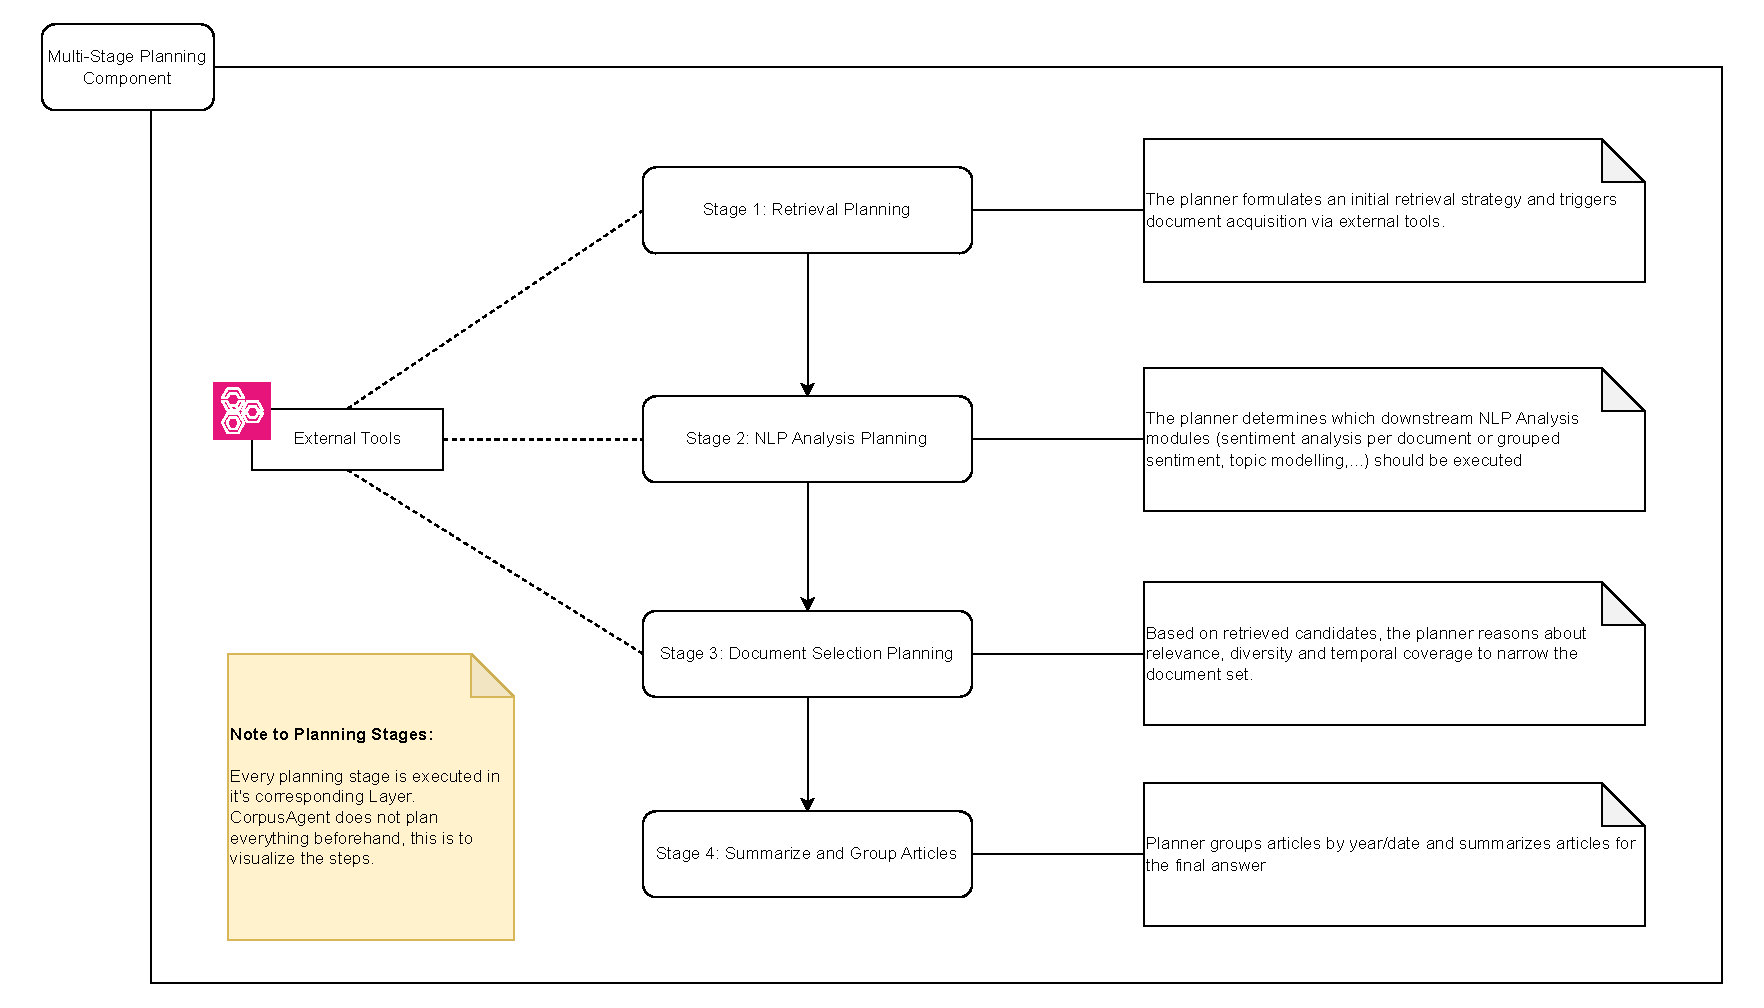
\includegraphics[width=1\textwidth]{Figures/planning-layer.pdf}
    \caption{Planning Layer}
    \label{fig:planning-layer}
\end{figure}

The Multi-Stage Planning Layer is responsible for orchestrating the overall problem-solving strategy of the CorpusAgent systeem. Contrary to the other layers, this layer is rather integrated into each of the other layers instead of being a standalone module as illustrated in Figure \ref{fig:planning-layer}. Rather than following a fixed, hard-coded execution path, this module introduces an agentic control mechanism in which a Large Language Model (LLM) dynamically determines how a given query should be processed across the various pipeline layers.

At this stage, the LLM is provided with a set of available external tools it can execute. These tools consist of function calls such as retrieval, natural language processing (NLP) analyses, document filtering and answer synthesis. However, the specific decisions regarding which tools to invoke, in what order and how many times are delegated to the LLM itself. Rather than a rigid sequence of operations, the planning layer enables a flexible, adaptive approach where the LLM can iteratively refine its strategy based on intermediate results. This design choice allows the system to adapt its strategy to the nature and complexity of the input query and can lead to multiple strategies for the same question.

What makes this approach particularly powerful is that the decision-making authority is not limited to a single planning step. Instead, the LLM is invoked after each major pipeline stage to reassess the current state of the task and determine the next best approach.

Each stage operates as a controlled execution step, while the overall reasing flow is handled by the LLM's conextual understanding ot the task. This agentic, multi-stage planning approach enables our system to handle a wide range of analytic queries with varying results. 

The first concrete execution step is determined by the LLM is the retrieval of the relevant documents, which is described in the next section.


\subsection{Retrieval Layer}

\begin{figure}[ht]
    \centering
    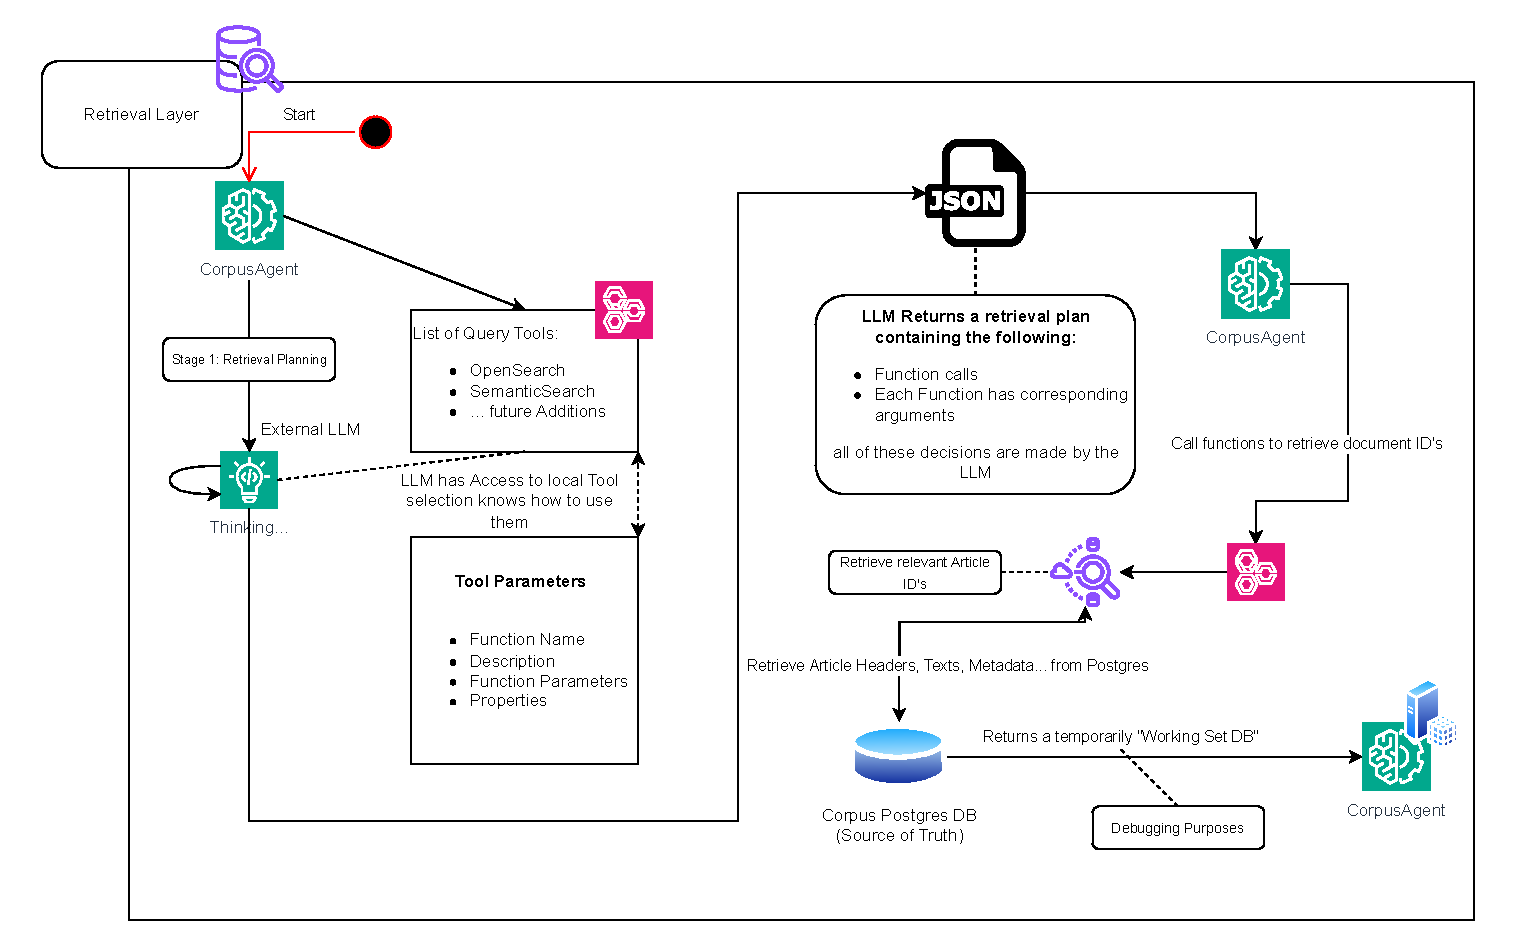
\includegraphics[width=1\textwidth]{Figures/retrieval-layer.pdf}
    \caption{Retrieval Layer}
    \label{fig:retrieval-layer}
\end{figure}

The Retrieval Layer is responsible for identifying and collecting a set of documents that are potentially relevant to the user’s query. Its primary goal is to efficiently reduce the overall corpus to a manageable subset that can be further analyzed by subsequent pipeline stages. An overview of this process is illustrated in Figure \ref{fig:retrieval-layer}.

As like with the other layers, the retrieval process is guided by the retrieval planning decisions made by the Large Language Model. The LLM determines here the appropriate retrieval strategy based on the user query and provided toolset. Rather than directly accessing the data itself, the LLM generates a structured retrieval plan in the form of one or more function calls. These function calls specify which retrieval tools should be used, the corresponding query expressions, and additional parameters such as the number of documents to return. All retrieval related decisions, including whether multiple retrieval calls are required, for example to cover different time periods, are made by the LLM.

Currently, the primary retrieval backend is OpenSearch, which is used to index the news corpus and enable fast full-text search. OpenSearch is based on the Lucene engine and relies on inverted indices, allowing keyword-based queries to be executed significantly faster than traditional relational database text matching. In preliminary experiments, this approach was empirically validated by comparing OpenSearch queries against SQL-based text search using \texttt{LIKE} expressions in PostgreSQL, where OpenSearch consistently produced substantially faster query execution times for large text collections. Which is to be expected given the underlying indexing mechanisms.

The use of OpenSearch at this stage is not only motivated by performance considerations but also by extensibility. The retrieval interface is designed in such a manner, such that additional retrieval mechanisms such as semantic vector search or alternative indexing systems can be integrated in the future without requiring fundamental changes to the architecture.

An example of a retrieval function call generated by the LLM is shown below:

\begin{lstlisting}[language=json, caption={Example OpenSearch retrieval function call}, label={lst:opensearch-call}]
{
  "id": "call_VBCxxwHwvAluJHuoMOrdC6iF",
  "type": "function",
  "function": {
    "name": "search_opensearch",
    "arguments": {
      "query": "Bitcoin (\"public perception\" OR \"public opinion\" OR sentiment OR adoption OR \"mainstream\" OR bubble OR scam OR regulation OR investment) 2016",
      "top_k": 50
    }
  }
}
\end{lstlisting}


\subsection{Analytics Layer}

The following section describes the Analytics Layer of the CorpusAgent system.

\subsection{Document Selection / Filtering Layer}

The following section describes the Document Selection / Filtering Layer of the CorpusAgent system.

\subsection{LLM Answer Synthesis}

The following section describes the LLM Answer Synthesis Layer of the CorpusAgent system.